\newpage
\section{Introduction to injections}
\genHeader
\hypertarget{sec:injections common}{}

This short introducion will show you how to implement small methods by adding handwritten code to classes created from your model. Injections are inspired by
partial classes in C\#, and are our preferred way of providing a clean separation between generated and handwritten code. 

Let's implement the \texttt{removeCard} method, declared in the \texttt{Partition} class. In order to `remove' a card from a partition, all one needs to do is
disable the link between them. Don't forget that (according to our signature) not only does \texttt{removeCard} have to pass in a \texttt{Card}, it must return
one as well.

\begin{itemize}


\item[$\blacktriangleright$] From your working set, open ``gen/LearningBoxLanguage.impl/PartitionImpl.java'' and enter the following code\footnote{To avoid
errors, you are able to copy/paste this text.} in the \texttt{removeCard} declaration, starting at approximately line 358. Do not remove the first comment,
which is necessary to indicate that this code is written by the user and needs to be extracted into our injection file.

\begin{figure}[htbp]
        \centering
        \begin{lstlisting}[language=Java, keywordstyle={\bfseries\color{purple}}, backgroundcolor=\color{white}]
    public Card removeCard(Card card) {
        // [user code injected with eMoflon]
        
        card.setCardContainer(null);
        return card;
    }
        \end{lstlisting}
        \caption{Implementation of \texttt{removeCard}}
        \label{fig:addToStringRep_impl}
\end{figure}

\item[$\blacktriangleright$] Save the file, then right-click on the file in the package explorer and choose ``eMoflon/ Create/Update Injection for class'' from
the context menu (Fig.~\ref{fig:injection_create_injection}).

\begin{figure}[htbp]
    \centering
    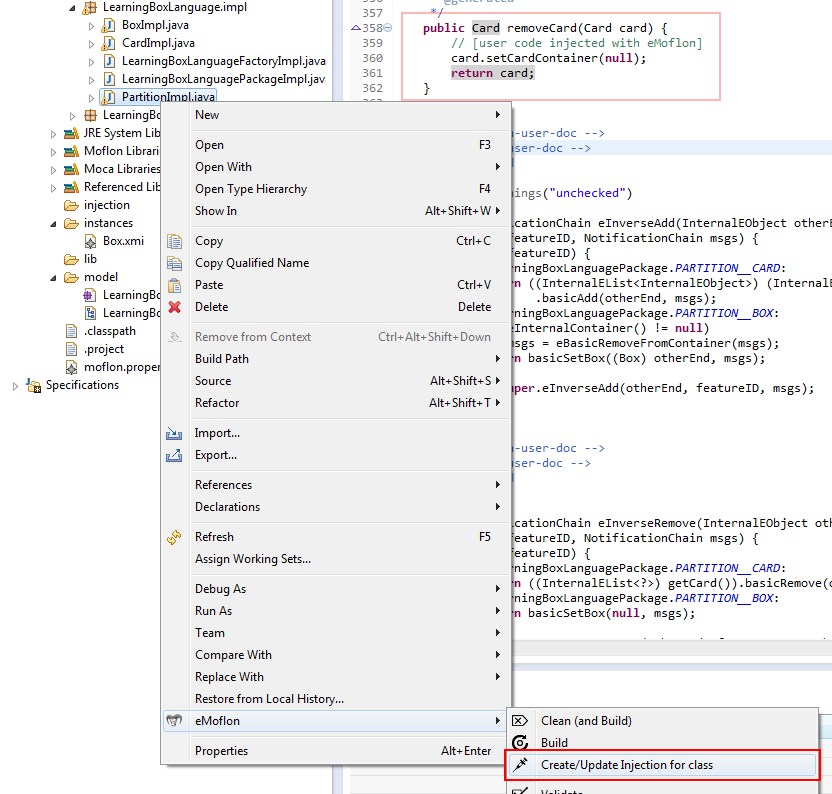
\includegraphics[width=\textwidth]{eclipse_createInjection}
    \caption{Create a new injection}
    \label{fig:injection_create_injection}
\end{figure}
    
\item[$\blacktriangleright$] This will create a new file in the ``injection'' folder of your project with the same package and name stucture as the Java class,
but with a new \texttt{.inject} extension (Fig.~\ref{fig:injection_folder}).

\begin{figure}[htbp]
    \centering
    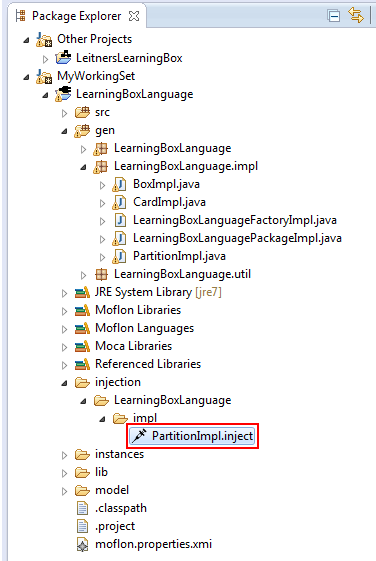
\includegraphics[width=0.5\textwidth]{eclipse_injectionFolder}
    \caption{Injection location}
    \label{fig:injection_folder}
\end{figure}

\item[$\blacktriangleright$] Double click to view this file. It contains the definition of a \textit{partial
class}~(Fig.~\ref{fig:injection_partialClassPartition}). Here you can see here the skeleton of two other functions you have the option of implementing in the
opposite direction. Instead of generating from the Java file, and injecting into its partial class, you could also generate the method contents from the
partial class, and inject it into its corresponding Java file.

\begin{figure}[htbp]
    \centering
    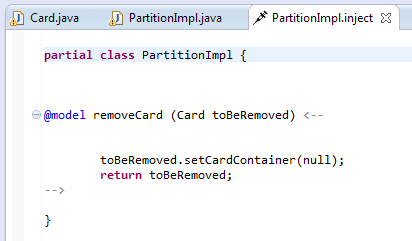
\includegraphics[width=0.9\textwidth]{eclipse_partialClass}
    \caption{Generated Injection file for \texttt{PartitionImpl.java}}
    \label{fig:injection_partialClassPartition}
\end{figure}

\clearpage

\item[$\blacktriangleright$] Lets try implementing a pair of methods in this alternate way. We reccommend the first as you can use the usual support
from the Java editor, but its always fun to learn.

\vspace{0.5cm}

\item[$\blacktriangleright$] Go to ``BoxImpl.java'' and, without editing any method signatures there, generate its corresponding injection file.

\vspace{0.5cm}

\item[$\blacktriangleright$] Another \texttt{.inject} file should have been placed in the same folder as \texttt{PartitionImpl.java}. Open this file, and notice
the partial class includes every method declaration but no implementation code (Fig.~\ref{fig:injection_partialClassBox}).

\vspace{0.5cm}

\begin{figure}[htbp]
    \centering
    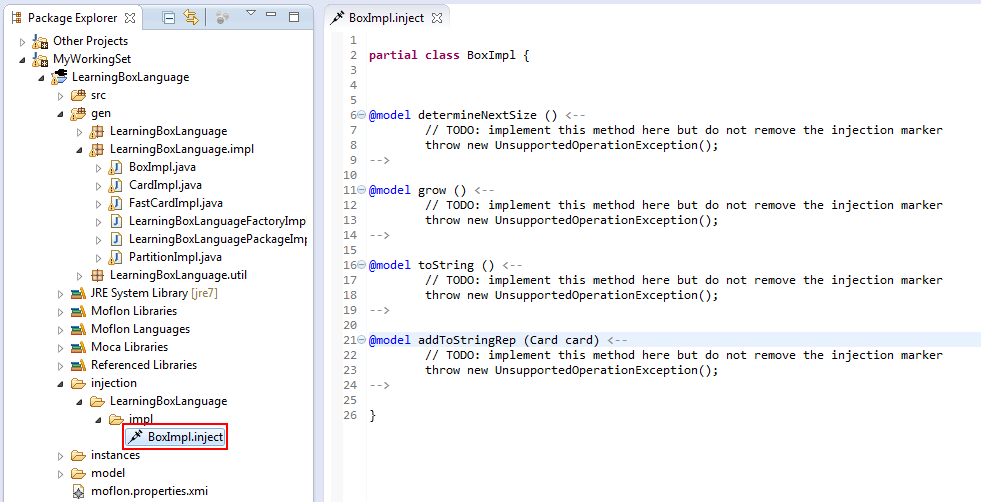
\includegraphics[width=1.0\textwidth]{eclipse_injectionBoxImpl}
    \caption{Generated Injection file for \texttt{BoxImpl.java}}
    \label{fig:injection_partialClassBox}
\end{figure}

\vspace{0.5cm}

\item[$\blacktriangleright$] Complete the \texttt{addToStringRep} and \texttt{determineNextSize} methods as specified in Fig.~\ref{code:complete_inject_file}

\begin{figure}[htbp]
        \centering
        \begin{lstlisting}[language=Java, keywordstyle={\bfseries\color{purple}}, backgroundcolor=\color{white}]
partial class BoxImpl {

    @model addToStringRep (Card card) <--

            StringBuilder sb = new StringBuilder();

            if (stringRep == null)
            {
                sb.append("BoxContent: [");

            }
            else
            {
                sb.append(stringRep);
                sb.append(", [");
            }

            sb.append(card.getFace());
            sb.append(", ");
            sb.append(card.getBack());
            sb.append("]");

            stringRep = sb.toString();
    -->

    @model determineNextSize () <--

            return getContainedPartition().size() * 10;
    -->

}
        \end{lstlisting}
        \caption{Implementation of helper methods as an injection}
        \label{code:complete_inject_file}
    \end{figure}
    \FloatBarrier

\item[$\blacktriangleright$] Right-click the injection file, and rebuild your project by selecting ``eMoflon/Clean and
Build''(Fig~\ref{fig:eclipse_buildFromInjecton}).

\vspace{0.5cm}

\begin{figure}[htbp]
    \centering
    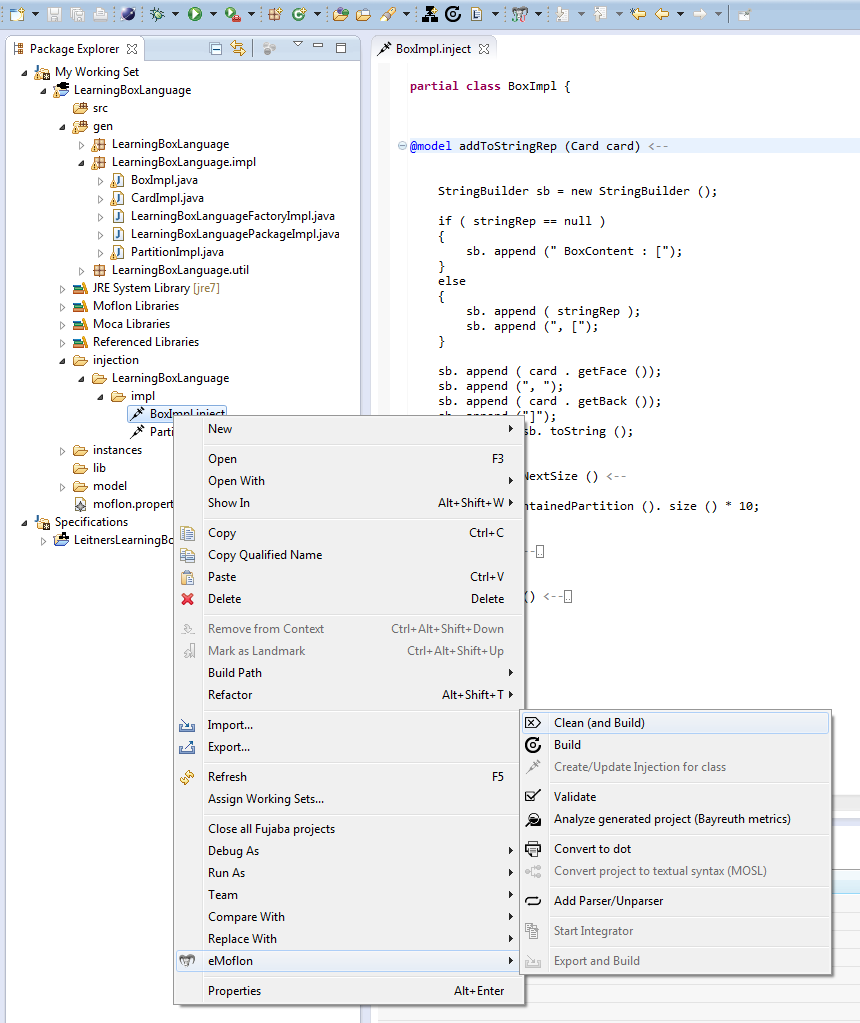
\includegraphics[width=1.0\textwidth]{eclipse_buildFromInject}
    \caption{Build the entire project from the injection file}
    \label{fig:eclipse_buildFromInjecton}
\end{figure}

\vspace{0.5cm}

\item[$\blacktriangleright$] The helper methods should now be implemented in the corresponding Java file (Fig~\ref{fig:eclipse_buildFromInjecton}).

\clearpage

\begin{figure}[htbp]
    \centering
    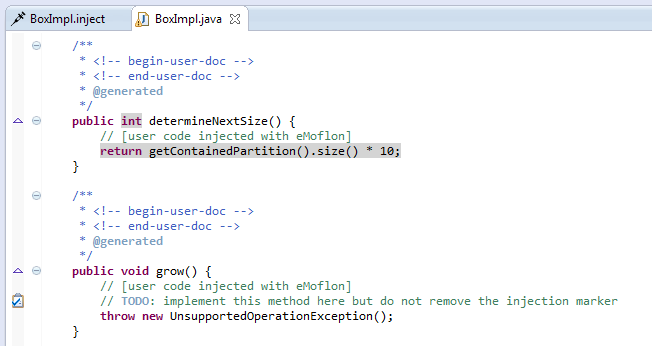
\includegraphics[width=1.0\textwidth]{eclipse_updatedBoxImpl}
    \caption{Update \texttt{BoxImpl.java} file}
    \label{fig:eclipse_updatedBoxImpl}
\end{figure}

\vspace{0.5cm}

\item[$\blacktriangleright$] For additional information on injections, check out Part IV Miscellaneous\footnote{\downLink} of the handbook.

\vspace{0.5cm}

\item[$\blacktriangleright$] While injecting in either direction is a remarkably simple process, it can quickly become challenging when trying to implement
complex functions. Instead, we'll learn how and continue to implement our method signatures with Story Diagrams in Part III.

 % \fancyfoot[R]{ $\triangleright$ \hyperlink{sec:LBGUI}{Next}}
 
\end{itemize}
